\documentclass[a4paper,12pt]{article}
\usepackage{amsmath}
\usepackage{graphicx}
\usepackage{fancyhdr}
\usepackage{placeins}
\usepackage{multirow}
\usepackage{geometry}
\usepackage{subcaption}
\usepackage{float}
\usepackage[bottom]{footmisc}
\geometry{top=1in, bottom=1in, left=1in, right=1in}
\usepackage{setspace}
\usepackage[style=bath,sorting=ynt]{biblatex}
\usepackage[hyperindex, colorlinks=true, linkcolor=blue, citecolor=blue]{hyperref}
\assignrefcontextentries[]{*}
\addbibresource{references.bib}
\RequireCitationStyle{authoryear-comp}
\ExecuteBibliographyOptions{uniquename=init}
\renewcommand*{\compcitedelim}{\addsemicolon\space}
\raggedbottom

\begin{document}

\pagestyle{fancy}  
\fancyhf{}  

%\setlength{\parindent}{0pt}
%\setlength{\parskip}{1em}  

\doublespacing  

% Adjust header height
\setlength{\headheight}{16pt}       
\addtolength{\topmargin}{-4pt}     


% Header setup
\fancyhead[C]{\fontsize{14}{16}\selectfont Belt Drive Lab Report}  

% Footer setup
\fancyfoot[R]{\thepage}

%TC:ignore
\begin{titlepage}
  \thispagestyle{empty}
  \centering
  
\includegraphics[width=0.6\textwidth]{uob-logo-grey-transparent-1.png} \\[2cm]
  {\Huge\textbf{Belt Drive Lab Report}} \\[1.5cm]
  {\LARGE\textbf{Department of Mechanical Engineering}} \\[0.5cm]
  {\LARGE\textbf{ME12005}} \\[1cm]
  {\Large\textbf{Student Name: Colin Peden}} \\[0.5cm]
  {\Large\textbf{Date: February 26, 2025}} \\[2cm]
  \vfill
\end{titlepage}

\begin{abstract}

\end{abstract}
%TC:endignore


\section{Introduction}
It is important to be able to predict the torque that can be transmitted by a belt drive system. Belt drives are commonly used due to their low cost and low maintenance requirements. Understanding the torque that can be transmitted by a belt allows for the calculation of power that can be transmitted and ensures that it is used in suitable systems. Belts can be characterised by measuring the tension ratio across a pulley with a given contact angle. Another variable in the system is the motor that drives it, as the torque transmitted varies, so does the efficiency of the motor and this should be characterised.

\subsection{Objectives}
To introduce techniques used for the characterisation of belt drive systems in order to: 


\begin{enumerate}
    \item Investigate the affect of contact angle ($\beta$) on the tension ratio.
    \item Investigate the relationship between the tension ratio and theoretical values at different contact angles ($\beta$).
    \item Calculate the coefficient of friction of the belt ($\mu$).
    \item Compare motor efficiency ($\eta$, \%) and torque ($\tau$, Nm).
\end{enumerate}

\section{Theory}
The theory used to govern the tension ratio of a belt between the tight side and the slack side ($T_1/T_2$) was initially discovered by Euler in 1775 (cite me) and then later expanded upon by Eytelwein in 1808 (cite me). The theory is given below: 

\begin{equation}
    \frac{T_2}{T_1} = e^{\mu \beta \sin\alpha}
    \label{eq:tension_ratio}
\end{equation}

where:
\begin{itemize}
    \item \( T_1 \) — Lower tension (Nm)
    \item \( T_2 \) — Higher tension (Nm)
    \item \( \alpha \) — Half of the V-belt angle
    \item \( \beta \) — Angle of contact between the belt and pulley
    \item \( \mu \) — Coefficient of friction
\end{itemize}

The V-belt angle ($\alpha$) for a flat belt as used in this experiment is 90° and so the $\sin\alpha$ term becomes 1 and can be disregarded.

The torque transmitted by a belt is given by the equation: 

\begin{equation}
    \tau = (T_2 - T_1) R
    \label{eq:torque}
\end{equation}]

where:
\begin{itemize}
    \item \( \tau \) — Torque transmitted by the belt (Nm)
    \item \( T_1 \) — Lower tension (N)
    \item \( T_2 \) — Higher tension (N)
    \item \( R \) — Pulley radius (m)
\end{itemize}

Power transmitted by the belt is then calculated by:

\begin{equation}
    P = \tau\omega
    \label{eq:power}
\end{equation}


where:
\begin{itemize}
    \item \(P\) - Power transmitted by the belt (W)
    \item \(\tau\) - Torque transmitted by the belt (Nm)
    \item \(\omega\) - Rotational speed of the pulley (rad/s)
\end{itemize}

Efficiency of the motor can be calculated by comparison of the output power from the equation above and the input power calculated from the current draw and the input voltage.

\section{Methods}
The apparatus for the experiment consisted of a DC motor with a variable speed driving an aluminium pulley with a fixed radius. A flat nylon belt is wrapped around the pulley, attached at its upper end to a load cell, and loaded with a series of weights at its other end. The contact angle ($\alpha$) can be varied through 4 set values and the weights vary in mass from 0.1-1kg in 0.1kg increments. The rotational speed ($\omega$) is measured using an optical tachometer, voltage and current are recorded from digital meters within the power supply.
A diagram detailing the apparatus is shown in Figure~\ref{fig:apparatus}


\begin{figure}[h]
    \centering
    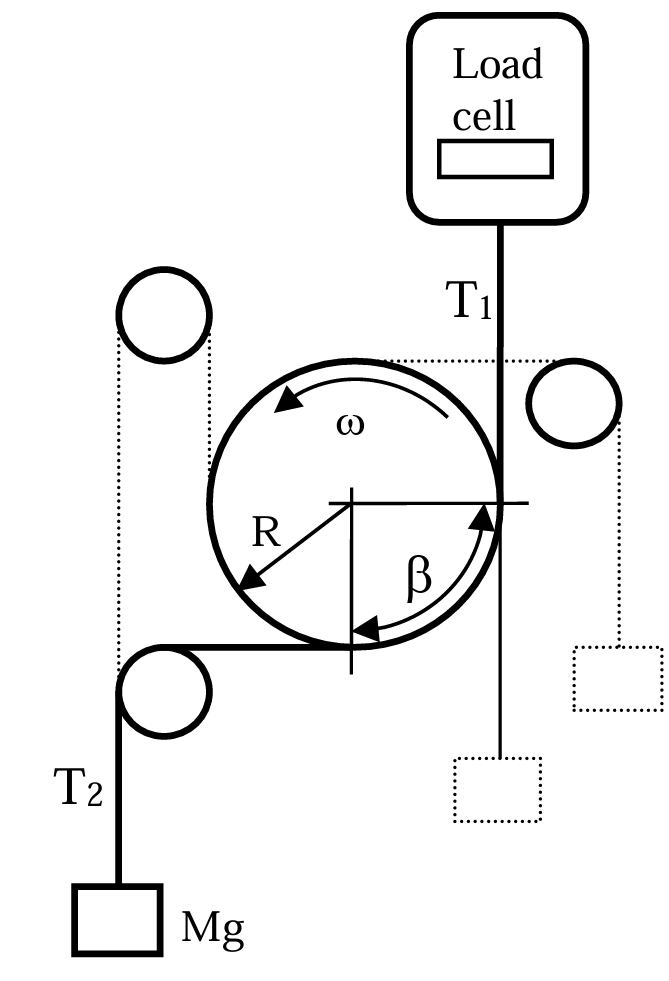
\includegraphics[width=0.4\textwidth]{figures/apparatus.png} 
    \caption{Experimental apparatus}
    \label{fig:apparatus}
\end{figure}

\break

\section{Results}
For each of the four wrap angles ($\alpha$) the recorded $T_1$ is plotted against $T_2$ and a line of best fit drawn, this is shown in Figure~\ref{fig:fig1}.

\begin{figure}[h]
    \centering
    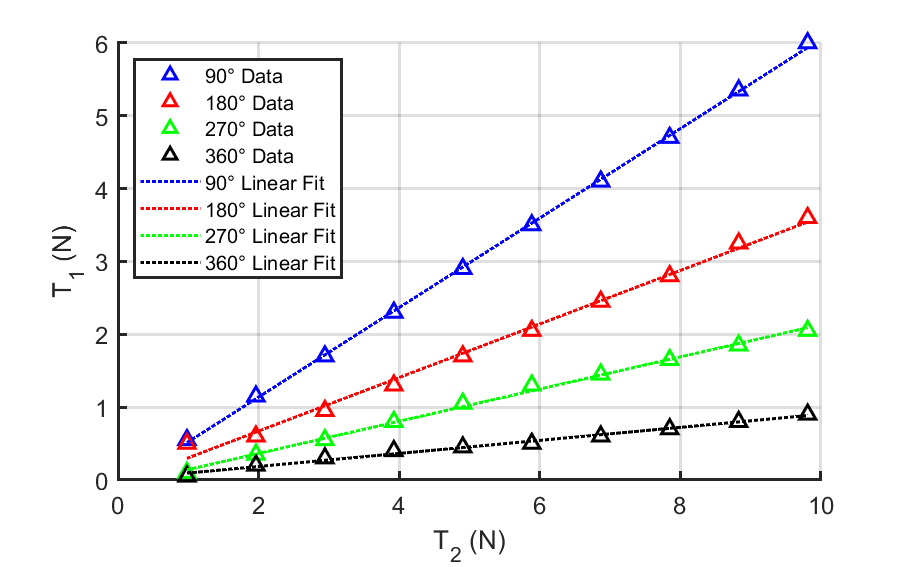
\includegraphics[width=0.9\textwidth]{figures/fig1.png}
    \caption{Plot of measured tensions, $T_1$ and $T_2$}
    \label{fig:fig1}
\end{figure}

The coefficient of friction ($\mu$) is calculated from ln($T_2/T_1$) and the contact angle ($\beta$). The tension ratios used are from the gradient of the linear fit models in Figure~\ref{fig:fig1}. This is plotted in Figure~\ref{fig:fig2} and $\mu$ can be taken as the gradient of the linear fit.

\begin{figure}[h]
    \centering
    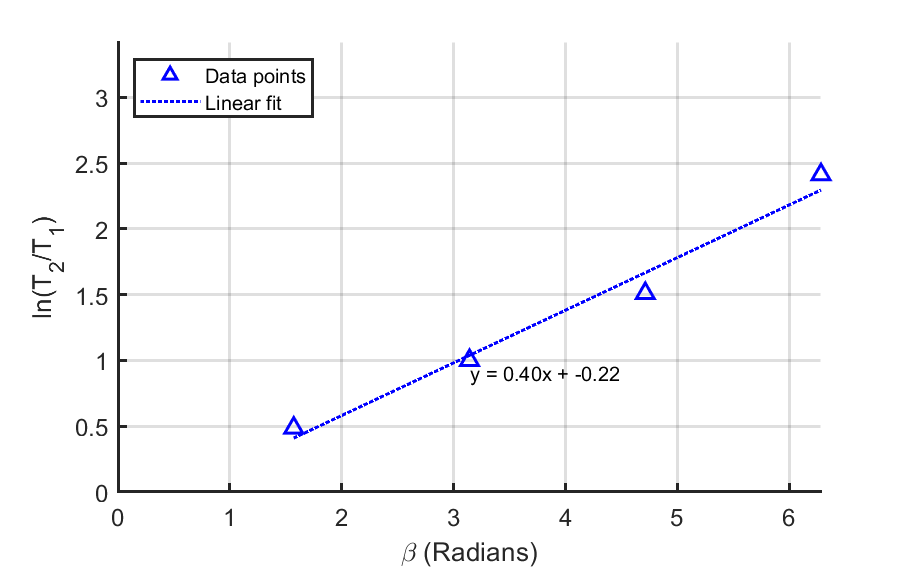
\includegraphics[width=0.9\textwidth]{figures/fig2.png}
    \caption{Plot of the natural logs of the tension ratios against contact angle ($\beta$)}
    \label{fig:fig2}
\end{figure}

\break

\section{Discussion}



\section{Conclusion}

\newrefcontext[sorting=nyt]
\printbibliography

\end{document}
